% 
% Lecture Template for ME3023 -  Measurements in Mechanical Systems - Tennessee Technological University
%
% Spring 2020 - Summer 2020
% Tristan Hill, May 07, 2020 - June 12, 2020 - July 08, 2020
% Module 7 - Time Varying Circuits
% Topic 3 - Frequency Filters
%

\documentclass{beamer} % for presentation (has nav buttons at bottom)
%\documentclass[handout]{beamer} % for handout 
\usepackage{beamerthemesplit}
\usepackage{listings}
\usepackage{multicol}
\usepackage{framed}
\usepackage{amsmath, nccmath}
\usepackage{geometry}
\usepackage{bm}

\beamertemplateballitem

% custom colors
\definecolor{TTUpurple}{rgb}{0.3098, 0.1607, 0.5176} % TTU Purple (primary)
\definecolor{TTUgold}{rgb}{1.0000, 0.8666, 0.0000} % TTU Gold (primary) 
\definecolor{mygray}{rgb}{.6, .6, .6}
\definecolor{mypurple}{rgb}{0.6,0.1961,0.8}
\definecolor{mybrown}{rgb}{0.5451,0.2706,0.0745}
\definecolor{mygreen}{rgb}{0, .39, 0}
\definecolor{mypink}{rgb}{0.9960, 0, 0.9960}

% color commands
\newcommand{\R}{\color{red}}
\newcommand{\B}{\color{blue}}
\newcommand{\BR}{\color{mybrown}}
\newcommand{\K}{\color{black}}
\newcommand{\G}{\color{mygreen}}
\newcommand{\PR}{\color{mypurple}}
\newcommand{\PN}{\color{mypink}}
\newcommand{\OR}{\color{orange}}
\newcommand{\GD}{\color{TTUgold}}


\setbeamercolor{palette primary}{bg=TTUpurple,fg=TTUgold}
\setbeamercolor{palette secondary}{bg=black,fg=TTUgold}
\setbeamercolor{palette tertiary}{bg=black,fg=TTUpurple}
\setbeamercolor{palette quaternary}{bg=TTUgold,fg=black}
\setbeamercolor{structure}{fg=TTUpurple} % itemize, enumerate, etc
\setbeamercolor{section in toc}{fg=TTUpurple} % TOC sections

%\usefonttheme{professionalfonts}

\newcommand{\Lagr}{\mathcal{L}} % lagrangian

\newcommand{\hspcu}{\underline{\hspace{20mm}}} % large horizontal space w underline
\newcommand{\vspccc}{\vspace{6mm}\\} % large vertical space
\newcommand{\vspcc}{\vspace{4mm}\\}   % medium vertical space
\newcommand{\vspc}{\vspace{2mm}\\}     % small vertical space

\newcommand{\hspcccc}{\hspace{10mm}} % large horizontal space
\newcommand{\hspccc}{\hspace{6mm}} % large horizontal space
\newcommand{\hspcc}{\hspace{4mm}}   % medium horizontal space
\newcommand{\hspc}{\hspace{2mm}}     % small horizontal space

\newcommand{\eqscl}{0.9}     % small horizontal space


\author{ME3023 - Measurements in Mechanical Systems} % original formatting from Mike Renfro, September 21, 2004

\newcommand{\MNUM}{7\hspace{2mm}} % Module number
\newcommand{\TNUM}{3\hspace{2mm}} % Topic number 
\newcommand{\moduletitle}{Time Varying Circuits}
\newcommand{\topictitle}{Frequency Filters} 

\newcommand{\sectiontitleI}{Signal, Amplitude, and Frequency}
\newcommand{\sectiontitleII}{Filter Concept}
\newcommand{\sectiontitleIII}{High-Pass, Low-Pass, and Band-Pass}
\newcommand{\sectiontitleIV}{Applications}

% custom box
\newsavebox{\mybox}

\title{Module \MNUM - \moduletitle}

\date{Mechanical Engineering\vspc Tennessee Technological University}

\begin{document}

\lstset{language=MATLAB,basicstyle=\ttfamily\small,showstringspaces=false}

\frame{\titlepage \center\begin{framed}\Large \textbf{Topic \TNUM - \topictitle}\end{framed} \vspace{5mm}}

% Section 0: Outline
\frame{
\large \textbf{Topic \TNUM - \topictitle} \vspace{3mm}\\

\begin{itemize}

	\item \sectiontitleI    \vspc % Section I
	\item \sectiontitleII 	\vspc % Section II
	\item \sectiontitleIII 	\vspc %Section III
	\item \sectiontitleIV 	\vspc %Section IV

\end{itemize}

}

% Section I:
\section{\sectiontitleI}

% Section I - Frame I:
\frame{
\frametitle{\sectiontitleI}

{\R Signal}, {\G Amplitude}, and {\B Frequency}\vspace{2mm}\\
\includegraphics[scale=.25]{amplitude_frequency.png} 
\includegraphics[scale=.25]{unit_circle.png}
					
What is the relationship between the unit circle and frequency?\vspace{5mm}\\


}


% Section I - Frame II:
\frame{ \small
\frametitle{\sectiontitleI}

\begin{multicols}{2}
Signals can be composed of multiple {\it frequency components}. \\ (see Fourier Analysis Ch2).\vspace{3mm}\\

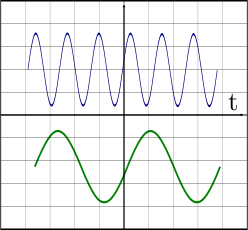
\includegraphics[scale=.4]{signal_addition.png}

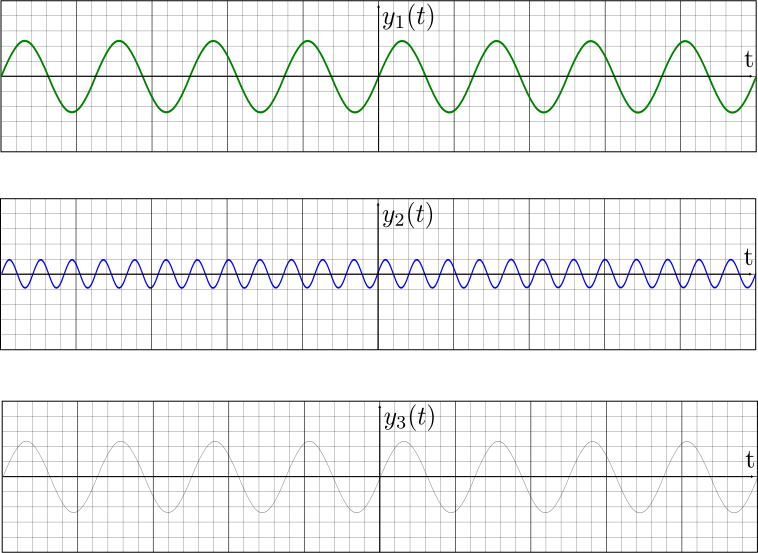
\includegraphics[scale=.30]{frequency_components.png}
\end{multicols}

}

% Section I - Frame III:
\frame{ \small
\frametitle{\sectiontitleI}


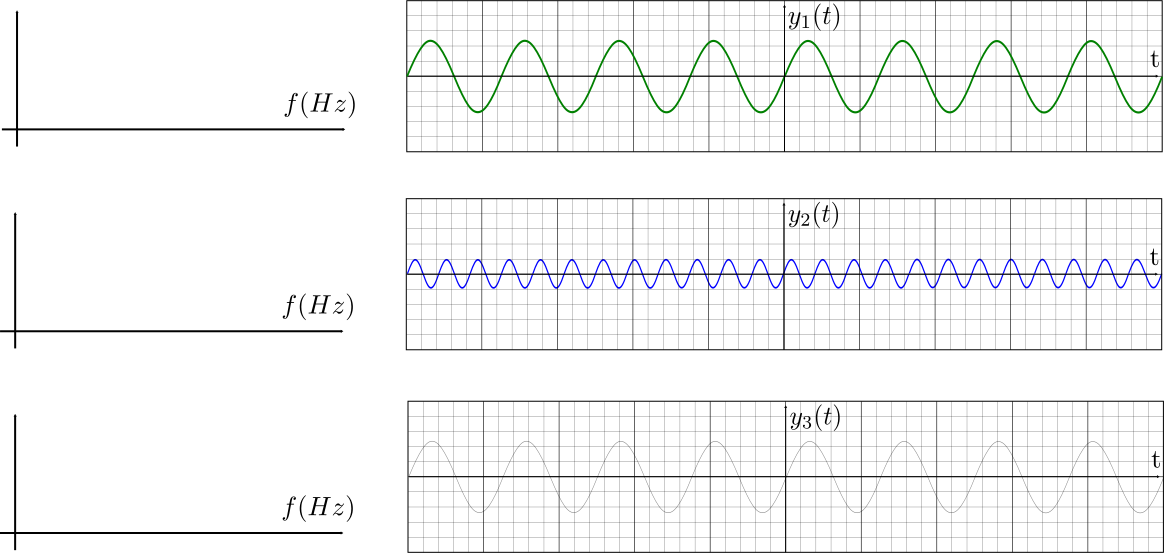
\includegraphics[scale=.35]{frequency_domain.png}

}




% Section II:
\section{\sectiontitleII}

% Section II - Frame I:
\frame{ \small
\frametitle{\sectiontitleII}

A {\PR raw signal} is input to a {\OR frequency filter} and a {\PN filtered signal} is output. \vspace{5mm}

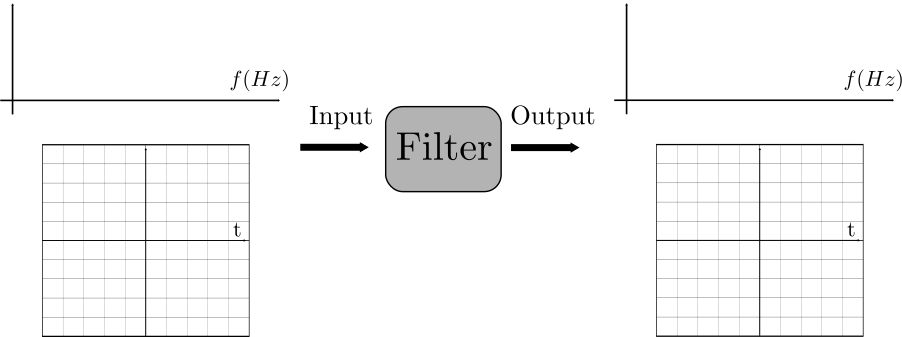
\includegraphics[scale=.45]{filter_concept.png}

} 

% Section II - Frame II:
\frame{
\frametitle{\sectiontitleII}

So what is inside the {\it grey box}? \vspace{10mm} \\

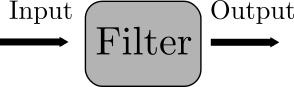
\includegraphics[scale=.5]{grey_box.png} \vspace{5mm} \\
How does it work? 

}


% Section II - Frame II:
\frame{
\frametitle{\sectiontitleII }

Filters are constructed from time-varying circuits. The most basic of which is the {\B RC filter}.
\begin{multicols}{2}

First Order Model
\[ \tau \dot{y}+y=KA \sin(\omega t) \]

Response Equation
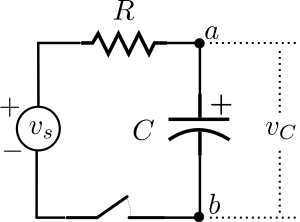
\includegraphics[scale=.5]{rc_circuit.png} \vspace{5mm} \\
\end{multicols}

\[ y(t)=Ce^{-\frac{t}{\tau}}+\frac{KA}{\sqrt{1+(\omega\tau)^2}}\sin(\omega t-\tan^{-1}(\omega\tau)) \]

}


% Section III:
\section{\sectiontitleIII}

% Section III - Frame I:
\frame{\small
\frametitle{\sectiontitleIII}
	
\includegraphics[scale=.25]{filter_types.png} \vspace{5mm} \\

}

% Section III - Frame II:
\frame{\small
\frametitle{\sectiontitleIII}
Physical frequency filters do not behave in an ideal manner as the previous figure shows. The filter characteristics are frequency dependent. 

\includegraphics[scale=.3]{bode_diagram.png} \vspace{5mm} \\

	
	
}

%% Section IV:
\section{\sectiontitleIV}

% Section IV - Frame I:
\frame{\small
\frametitle{\sectiontitleIV}

	
	Finally, what are filters used for? 
	\begin{itemize}
		\item 
		\item 
		\item	
	\end{itemize}

}
	
\end{document}



